\chapter{Experiments and Results}

During the Tunnel Circuit, we deployed our complete system, comprising 2 ground robots (R1, R2) and a drone (D1) a total of 4 times over 4 days. For the 1st and 4th days, we operated in the Experimental mine, while on the 2nd and 3rd days we operated in the Safety Research Mine. The second run for each mine had a different set of artifacts and locations than the first. The final scores for each deployment, as recorded by DARPA, are shown in Table \ref{final_scores}. Each configuration had 20 artifacts deployed.

\begin{table}
	\centering
	\begin{adjustbox}{max width=.95\textwidth}
		\csvreader[
		respect underscore=true,
		tabular=|l|l|c|c|,
		late after line=\\\hline,
		table head=\hline \textbf{Date} & \textbf{Course Name} & \textbf{Artifact Configuration} & \textbf{Official Score}\\\hline,
		]{final_scores.csv}{}{\csvlinetotablerow}
	\end{adjustbox}
	\caption{Official scores from Tunnel Circuit}
	\label{final_scores}
\end{table}

\section{Experimental Setup}

After the Tunnel Circuit, a number of experiments were performed to determine the utility and performance of each part of the system. All experiments were performed by playing back data recorded on R2  (which carried the Mk. 1 payload) on day 2, in the Safety Research mine with artifact configuration A. Ground truth artifact locations for this configuration were obtained by transforming the ground truth provided by DARPA after the competition into R2's /map frame using the calibration determined at competition. The calibration was not updated between experiments. This transformation allowed all experiments to take place in R2's /map frame, rather than requiring a transformation of artifact coordinates during experiments. A map of the Safety Research mine, artifact locations, as well as the areas traversed by R2 on day 2 is given in Figure \ref{tunnel_circuit_day_2}.

\begin{figure}	
	\centering
	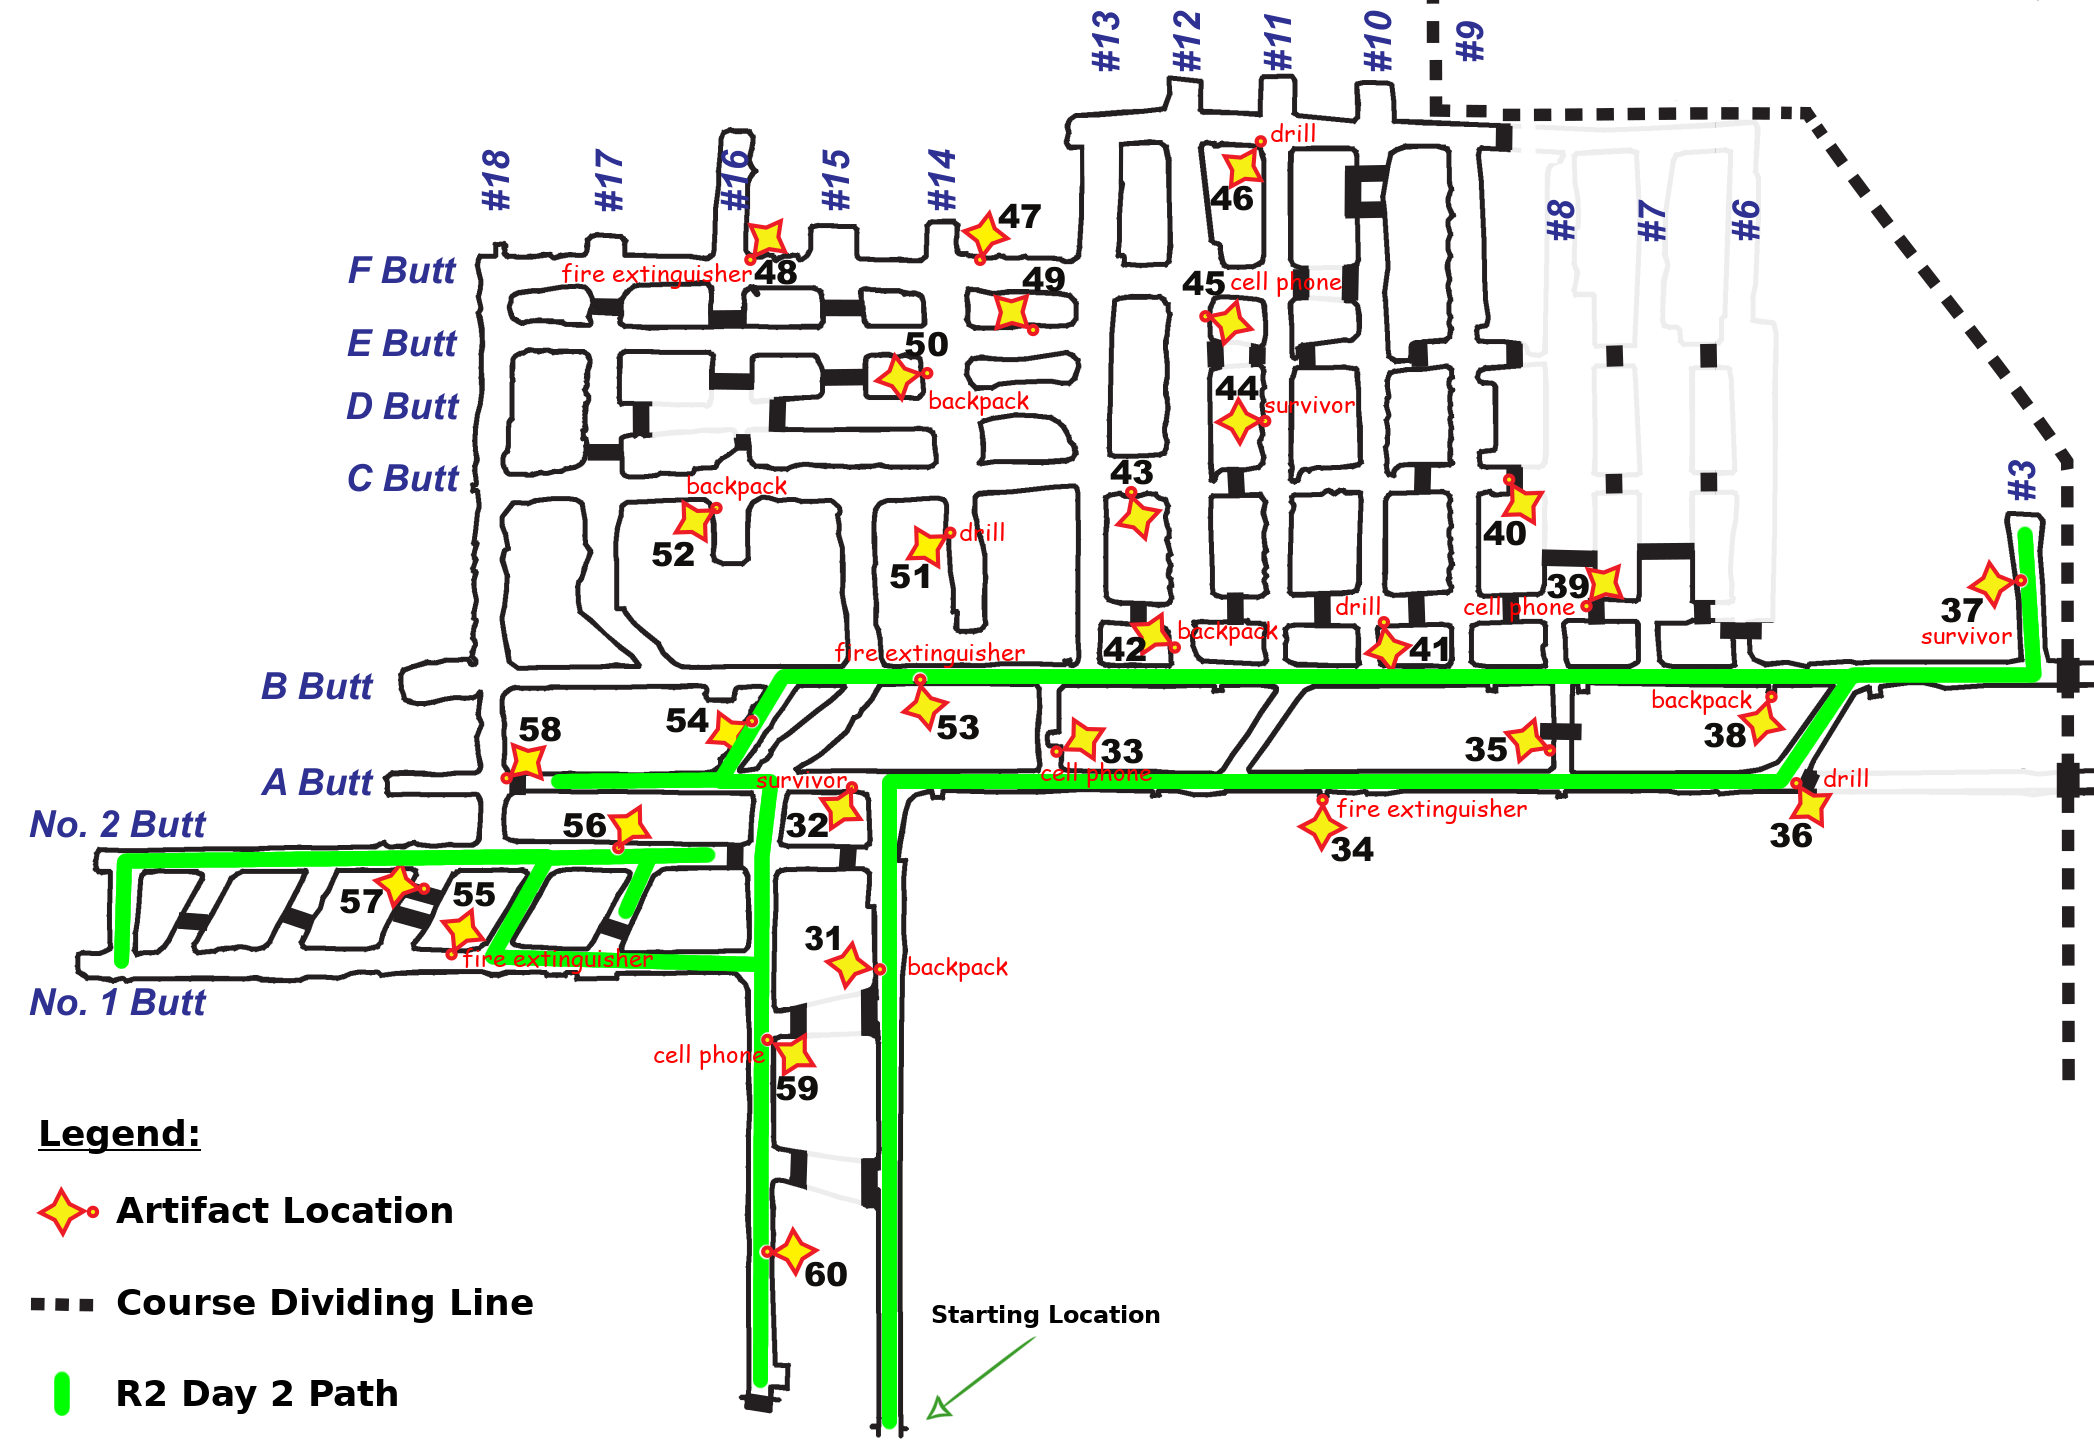
\includegraphics[width=\textwidth]{Tunnel_Artifact_Map_day_2.png}
	\caption[Tunnel Circuit day 2 artifact locations]{Ground truth locations for artifacts in the Safety Research mine during day 2 of the Tunnel Circuit. Numbers with text represent locations where artifacts were actually present. Locations without text did not contain artifacts. The cell phone at location 33 was not broadcasting an access point during this day due to a confirmed error by DARPA. The robot started at the right tunnel in the center of the figure and turned around after reaching No. 1 Butt after approximately 20 minutes.}
	\label{tunnel_circuit_day_2}
\end{figure}

During each experiment, the system reported artifacts directly to a scoring server, rather than reporting them to the base station for human verification. While this setup is slightly different than that used during competitions, it enables more consistent and repeatable experiments and allows multiple experiments to be run in parallel. The scoring server aggregates all artifacts reported by the system similarly to other nodes, and scores the entire list of artifacts whenever an update is received. Artifacts are scored by matching valid artifacts to ground truth artifacts, ensuring that the reported artifact is within 5m Euclidean distance of the ground truth artifact and shares the same class. Precision is determined according to Equation \ref{precision_equation}. The results are appended to a file on disk, allowing the system's performance over time to be analyzed.

\begin{equation} \label{precision_equation}
precision = \frac{\#\ correct\ artifacts}{\#\ valid\ artifacts}
\end{equation}

Streaming results directly to the server also removes the effect of communication network, assuming instead that the robot is always able to communicate with the base station. An analysis of the actual bandwidth usage under different configurations of the artifact compressor for the R2 day 2 dataset is given in Figure \ref{bandwidth_usage}. 

The results of each experiment are compared to the results of the configuration used during the Tunnel Circuit, described in Figure \ref{software_overview}. Values in plots indicating the number of artifacts detected have been slightly altered by adding an offset of between -3\% and 3\% to all values to improve legibility. Values in all other plots have not been altered.

\section{Single Sensor Usage}

Our core hypothesis for this work is that the use of multiple sensors and sensing modalities is necessary and advantageous in detecting and localizing artifacts. To test this hypothesis, as well as to understand the utility of each individual sensor, the artifact detection and localization pipeline was run with only a single sensor active at once. Each of the 4 RGB cameras and 2 thermal cameras were run separately, while both radios feeding the signal localizer were run simultaneously. The results are shown alongside the full system with all sensors active simultaneously in Figure \ref{sensors_vs_full}.

\begin{figure}	
	\centering
	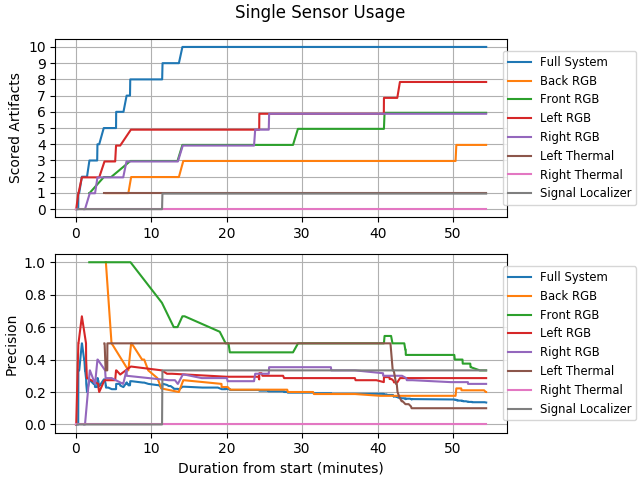
\includegraphics[width=\textwidth]{eval_graphs/sensors_vs_full.png}
	\caption[Single sensor artifact localization]{The plot shows the results from configurations in which only a single sensor was active. Both radios were used simultaneously for the signal localizer.}
	\label{sensors_vs_full}
\end{figure}

When combining all of the sensors, the robot was able to score all 10 artifacts in its path by approximately 15 minutes. No single sensor was able to achieve the same score, even at the end of the competition run. A total of 9 artifacts could have been detected by each RGB camera, which is all artifacts except the cell phone at location 59 in Figure \ref{tunnel_circuit_day_2}. Each RGB camera scored most, but not all, of the artifacts in the robot's path, and required the robot to turn around and back to the entrance of the tunnel, which happened at approximately 20 minutes into the run. Using the full system, the robot would instead be able to keep exploring and continue to report information for situational awareness. 

Two survivor artifacts were present along the robot's path which could have been detected by the thermal cameras. When using only the left thermal camera, only 1 survivor artifact was scored. None were scored by the right thermal camera. This may be attributed to a lower quality thermal object detector as a result of fewer training examples, or the low framerate of thermal detection (5 Hz) preventing sufficient confidence from accumulating to consider a detected object an artifact.

The signal localizer is the only module capable of localizing cell phones, and was able to score the single cell phone artifact (59) acting as a WiFi access point along its path (59). The other two broadcasting cell phone artifacts (39, 45) were detected by the WiFi scanner but could not be localized sufficiently accurately by the signal localizer since the robot did not traverse the areas near the artifacts.

While each individual sensor had a lower overall score than the complete system, all sensors except the thermal cameras resulted in a higher precision than the overall system. This may be due to the fact that all configurations used the same confidence thresholds for determining when to publish an Artifact Localization. When only a single sensor is used, more false positive detections are required per sensor to create a false positive Artifact Localization than when all sensors are fused together. The higher false positive rate for the full system is acceptable based on the team's concept of operations, but this experiment may indicate an opportunity to lower the false positive rate by dynamically adapting confidence thresholds based on the number of sensors being fused.

\section{RealSense Depth Only}

During the development process, we discovered that the RealSense camera's depth accuracy drops significantly after approximately 2.5m. As a result, depth information from the RealSense is discarded after 2.5m and replaced with depth information from the LIDAR in the full system. This experiment quantifies the utility of the fusion of LIDAR data by examining the system performance with only a single RealSense activated and limited to using only RealSense depth information under 2.5m. The results are shown in Figure \ref{rs_depth_only}.

\begin{figure}	
	\centering
		\begin{subfigure}{0.48\textwidth}
			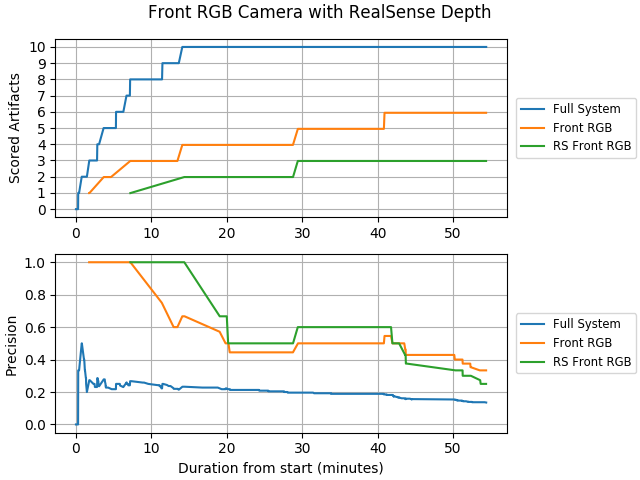
\includegraphics[width=\textwidth]{eval_graphs/rs_depth_front.png}
			\label{rs_depth_front}
		\end{subfigure}
		\hfill
		\begin{subfigure}{0.48\textwidth}
			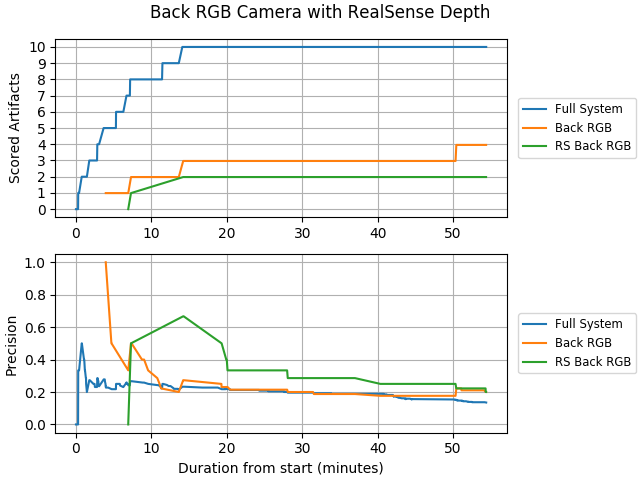
\includegraphics[width=\textwidth]{eval_graphs/rs_depth_back.png}
			\label{rs_depth_back}
		\end{subfigure}
		\\
		\begin{subfigure}{0.48\textwidth}
			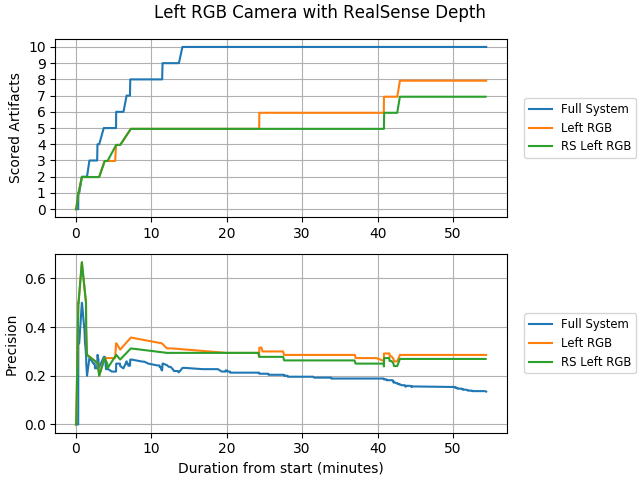
\includegraphics[width=\textwidth]{eval_graphs/rs_depth_left.png}
			\label{rs_depth_left}
		\end{subfigure}
		\hfill
		\begin{subfigure}{0.48\textwidth}
			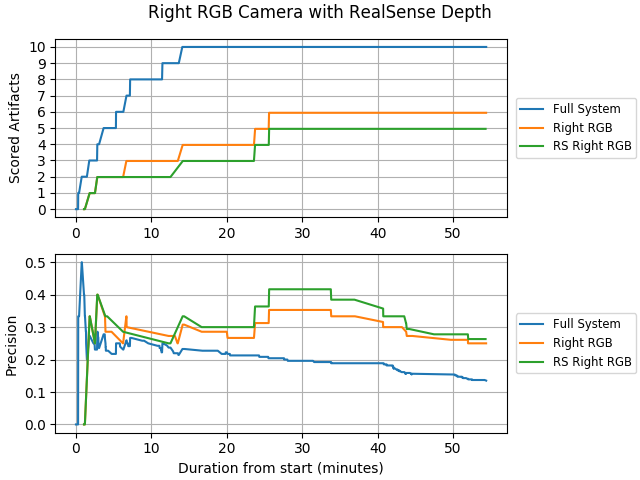
\includegraphics[width=\textwidth]{eval_graphs/rs_depth_right.png}
			\label{rs_depth_right}
		\end{subfigure}
	\caption[Single RGB sensor scores using only RealSense depth]{Only the RealSense depth information was used to localize artifacts in this test, resulting in an effective detection range of 2.5m for the RGB cameras.}
	\label{rs_depth_only}
\end{figure}

The front and back cameras have the largest decrease in accuracy when utilizing only RealSense depth information, with each scoring only half of the artifacts scored when fusing LIDAR information. This is likely due to the topology of the environment itself. The Tunnel Circuit environment consists of many narrow corridors. When the robot drives by artifacts and they are detected by the left and right RGB cameras, the artifact is typically very close to the robot. In contrast, the front and back cameras are typically looking down the long corridors and thus artifacts are often beyond the 2.5m threshold. The precision of each of the RGB cameras with both types of depth information is comparable and significantly higher than that of the full system.
